%%%% CAPÍTULO 4 - RESULTADOS E DISCUSSÃO

\chapter{Resultados}\label{cap:resultados}

Este capítulo descreve os resultados preliminares do trabalho, que é um cliente \textit{web}, com foco no controle de gestão de propriedades rurais, acompanhamento de animais nas propriedades rurais e gerenciamento financeiro da propriedade, entre outras funcionalidades.

Em seguida, será abordado o escopo, destacando as principais funcionalidades e os atores envolvidos. Em seguida, abordaremos a modelagem do sistema, que compreende a definição dos requisitos funcionais e não funcionais, juntamente com a elaboração dos diagramas de casos de uso e do modelo de entidade e relacionamento do banco de dados.

\section{Escopo do sistema}\label{sec:escopoSistema}

O cliente \textit{web} para gerenciamento de gado leiteiro será principalmente utilizado por técnicos do \gls{IDR-PR}. Sendo a principal finalidade o controle e manuseio dos dados, a fim de evitar incoerência nos registros coletados. A plataforma \textit{web} consumirá dados de uma \gls{API} \gls{REST} que está em desenvolvimento e manutenção em paralelo ao desenvolvimento deste trabalho.

Cada técnico poderá fazer o gerenciamento dos dados da propriedade vinculado, bem como dados do rebanho, dados financeiros, dados de insumos e produtos e dados de plantações.

O sistema iniciará com uma página de autenticação, caso o técnico ainda não possua cadastro ele poderá cadastrar-se. Vale ressaltar que uma propriedade pode ser relacionada a um ou mais técnicos, os técnicos só poderão analisar dados das propriedades em que estão vinculados. Estão incluídos no sistema além de cadastro e autenticação do técnico, o módulo de propriedades, módulo financeiro, módulo de animais, produtos e insumos e o módulo de plantações, sendo que exceto o módulo de propriedade, os demais são sempre referentes a uma propriedade.

No módulo dedicado às propriedades, serão cadastrados diversos dados importantes, incluindo informações sobre o produtor, colaboradores, a área destinada à bovinocultura (em hectares), coordenadas de localização e uma imagem representativa da propriedade.

Na seção voltada aos animais, serão registradas informações abrangentes, tais como dados sobre partos, inseminações, casos de mastite, doenças, medicamentos administrados, diagnósticos de prenhez, além de detalhes sobre vendas, compras e óbitos de animais.

No módulo relacionado às plantações, haverá um controle rigoroso sobre informações envolvendo pragas e doenças, abrangendo a identificação da cultura afetada, o tipo de praga ou doença identificada e o grau de infestação presente.

No que concerne ao módulo financeiro, serão meticulosamente gerenciados registros de receitas e despesas. Tais registros incluirão datas, tipos, quantidades, valores expressos em reais e descrições detalhadas, com a possibilidade de realizar agrupamentos para uma análise mais precisa.

No módulo de produtos e insumos, os usuários terão a capacidade de controlar detalhes referentes aos produtos utilizados, quantidade empregada, data de aplicação e o propósito da utilização específica.

Dessa maneira, todas as informações referentes à uma propriedade rural serão armazenadas e servirão como subsídio para que os técnicos possam auxiliar na melhora da produtividade dessas propriedades.


\section{Modelagem do sistema}\label{sec:modelagemSistema}

Nesta seção, são delineados os requisitos funcionais e não funcionais, os casos de uso e os diagramas que descrevem pormenorizadamente os processos e a estrutura do sistema a ser desenvolvido. Cada requisito funcional é introduzido, seguido dos requisitos não funcionais pertinentes.
Os requisitos funcionais são detalhados entre o \autoref{quad:requisitoCadastroUsuario} até o \autoref{quad:requisitoCadastroProdutor}, enquanto os requisitos não funcionais são apresentados nos quadros correspondentes, do \autoref{quad:requisitoCadastroUsuario} até o \autoref{quad:requisitoCadastroProdutor}, respectivamente.

\subsection{Requisitos funcionais e não funcionais}\label{subsec:requisitosFuncionaisNaoFuncionais}

No \autoref{quad:requisitoCadastroUsuario} é apresentado o requisito funcional de Cadastro de Usuário, que é fundamental para habilitar o acesso aos diferentes módulos do sistema. Os requisitos não funcionais relacionados a este requisito descrevem os dados necessários para efetuar o registro do usuário, incluindo informações relevantes ao processo de criação da conta.

\begin{tabframed}[htb]
  \caption{Cadastro do usuário}
  \label{quad:requisitoCadastroUsuario}
  \renewcommand{\arraystretch}{1.5}
  \begin{tabular}{|l|l|}
    \cline{1-2}
    \multicolumn{2}{|l|}{\textbf{F1 - Cadastro do usuário} }
    \\ \cline{1-2}

    \multicolumn{2}{|p{15cm}|}{
    \raggedright \textbf{Descrição:} O sistema deve permitir o cadastro de usuários para acesso ao sistema. O sistema deve apresentar os Termos de Uso durante o processo de cadastro. O usuário deve ser capaz de ler os Termos de Uso de forma clara. Deve haver uma opção clara para que o usuário aceite os Termos de Uso. O sistema deve solicitar as informações necessárias para criar um usuário, incluindo nome completo, CPF, município, CEP, rua, telefone, email, registro profissional e ano de formatura.
    }
    \\ \cline{1-2}

    \multicolumn{2}{|l|}{\textbf{Requisitos Não-Funcionais}}
    \\ \cline{1-2}

    \textbf{Nome}                  &
    \textbf{Restrição}
    \\ \cline{1-2}

    NF 1.1 Segurança de Dados      &
    \multicolumn{1}{|p{8cm}|}{\raggedright Os dados dos usuários, incluindo informações pessoais e aceitação dos Termos de Uso, devem ser armazenados de forma segura e protegidos contra acesso não autorizado.}
    \\ \cline{1-2}

    NF 1.2 Validações ao cadastrar &
    \multicolumn{1}{|p{8cm}|}{\raggedright O sistema deve validar os dados informados pelo usuário e não deve permitir cadastro em situações de email ou CPF já existente.}
    \\ \cline{1-2}

    NF 1.3 Usabilidade             &
    \multicolumn{1}{|p{8cm}|}{\raggedright O processo de cadastro deve ser intuitivo e fácil de ser realizado, com instruções claras para o usuário. O sistema deve fornecer feedback imediato em caso de erros ou campos obrigatórios não preenchidos.}
    \\ \cline{1-2}
  \end{tabular}
  \fonte{} % Fonte
\end{tabframed}

No \autoref{quad:requisitoNiveisAcesso}, apresenta-se o requisito funcional de Níveis de Acesso, um componente essencial para a estrutura de autorização e controle de acesso do sistema. Esse requisito é fundamental para garantir que os usuários tenham acesso apenas às informações pertinentes às suas funções e responsabilidades no sistema. Os diferentes níveis de acesso são definidos com base nas permissões específicas de cada tipo de usuário.

\begin{tabframed}[htb]
  \caption{Níveis de Acesso}
  \label{quad:requisitoNiveisAcesso}
  \renewcommand{\arraystretch}{1.5}
  \begin{tabular}{|l|l|}
    \cline{1-2}
    \multicolumn{2}{|l|}{\textbf{F2 - Níveis de Acesso}}
    \\ \cline{1-2}

    \multicolumn{2}{|p{15cm}|}{
    \raggedright \textbf{Descrição:} O sistema deve estabelecer níveis de acesso, cada um com suas respectivas permissões para visualização e gerenciamento de dados.
    }
    \\ \cline{1-2}

    \multicolumn{2}{|l|}{\textbf{Requisitos Não Funcionais}}
    \\ \cline{1-2}

    \textbf{Nome}                     &
    \textbf{Restrição}
    \\ \cline{1-2}

    NF 2.1 Segurança de Acesso        &
    \multicolumn{1}{|p{8cm}|}{\raggedright O sistema deve garantir a segurança das informações, permitindo apenas o acesso de usuários autorizados, de acordo com seu nível.}
    \\ \cline{1-2}

    NF 2.2 Auditoria de Acesso        &
    \multicolumn{1}{|p{8cm}|}{\raggedright Deve haver um registro de todas as ações realizadas por usuários em diferentes níveis de acesso, permitindo a auditoria e rastreamento.}
    \\ \cline{1-2}

    NF 2.3 Desempenho Eficiente       &
    \multicolumn{1}{|p{8cm}|}{\raggedright O sistema deve manter tempos de resposta rápidos, independentemente do nível de acesso, garantindo eficiência na gestão e recuperação de dados.}
    \\ \cline{1-2}

    NF 2.4 Customização de Permissões &
    \multicolumn{1}{|p{8cm}|}{\raggedright A flexibilidade do sistema permite que administradores atribuam permissões personalizadas de acordo com as necessidades.}
    \\ \cline{1-2}
  \end{tabular}
  \fonte{} % Fonte
\end{tabframed}

No \autoref{quad:requisitoAutenticacaoUsuario} é exibido o requisito funcional de Autenticação do Usuário, um requisito necessário para acessar os demais módulos do sistema. Nos requisitos não funcionais associados a este requisito, são detalhados os dados utilizados no processo de autenticação (\textit{login}).

\begin{tabframed}[htb]
  \caption{Autenticação do Usuário}
  \label{quad:requisitoAutenticacaoUsuario}
  \renewcommand{\arraystretch}{1.5}
  \begin{tabular}{|l|l|}
    \cline{1-2}
    \multicolumn{2}{|l|}{\textbf{F3 - Autenticação do Usuário}}
    \\ \cline{1-2}

    \multicolumn{2}{|p{15cm}|}{
    \raggedright \textbf{Descrição:} O sistema deve fornecer um mecanismo de autenticação de usuário para permitir o acesso aos diferentes módulos do sistema. A autenticação é um requisito fundamental para garantir a segurança e a identificação dos usuários.
    }
    \\ \cline{1-2}

    \multicolumn{2}{|l|}{\textbf{Requisitos Não Funcionais}}
    \\ \cline{1-2}

    \textbf{Nome}                    &
    \textbf{Restrição}
    \\ \cline{1-2}

    NF 3.1 Segurança na Autenticação &
    \multicolumn{1}{|p{8cm}|}{\raggedright O sistema deve garantir que o processo de autenticação seja seguro, protegendo as informações de login e senha contra acessos não autorizados.}
    \\ \cline{1-2}

    NF 3.2 Usuários Autorizados      &
    \multicolumn{1}{|p{8cm}|}{\raggedright A autenticação deve permitir o acesso apenas a usuários devidamente autorizados e cadastrados, verificando as credenciais de login.}
    \\ \cline{1-2}
  \end{tabular}
  \fonte{} % Fonte
\end{tabframed}

No \autoref{quad:requisitoManterPropriedades} é apresentado o requisito funcional denominado "Manter Propriedades". Este requisito é essencial para o funcionamento adequado dos demais módulos do sistema, uma vez que serve como o cadastro fundamental para as operações subsequentes. Nos requisitos não funcionais associados a este requisito, são estabelecidas diretrizes e restrições adicionais que impactam a forma como as propriedades são mantidas no sistema, garantindo a eficiência, segurança e controle necessários.

\begin{tabframed}[htb]
  \caption{Manter Propriedades}
  \label{quad:requisitoManterPropriedades}
  \renewcommand{\arraystretch}{1.5}
  \begin{tabular}{|l|l|}
    \cline{1-2}
    \multicolumn{2}{|l|}{\textbf{F4 - Manter Propriedades}}
    \\ \cline{1-2}

    \multicolumn{2}{|p{15cm}|}{
    \raggedright \textbf{Descrição:} O sistema deve disponibilizar funcionalidades para a manutenção de propriedades, o que inclui a inserção, atualização e recuperação de informações relacionadas às propriedades. Esse requisito é de vital importância para a operação adequada de todos os módulos do sistema, uma vez que serve como a base de dados central.
    }
    \\ \cline{1-2}

    \multicolumn{2}{|l|}{\textbf{Requisitos Não Funcionais}}
    \\ \cline{1-2}

    \textbf{Nome}                         &
    \textbf{Restrição}
    \\ \cline{1-2}

    NF 4.1 Segurança de Acesso            &
    \multicolumn{1}{|p{8cm}|}{\raggedright O sistema deve garantir a segurança das informações, permitindo apenas o acesso de usuários autorizados, de acordo com seu nível.}
    \\ \cline{1-2}

    NF 4.2 Auditoria de Acesso            &
    \multicolumn{1}{|p{8cm}|}{\raggedright Deve haver um registro de todas as ações realizadas por usuários em diferentes níveis de acesso, permitindo a auditoria e rastreamento.}
    \\ \cline{1-2}

    NF 4.3 Desempenho Eficiente           &
    \multicolumn{1}{|p{8cm}|}{\raggedright O sistema deve manter tempos de resposta rápidos, independentemente do nível de acesso, garantindo eficiência na gestão e recuperação de dados.}
    \\ \cline{1-2}

    NF 4.4 Correlacionamento com Produtor &
    \multicolumn{1}{|p{8cm}|}{\raggedright O sistema deve disponibilizar formas de correlacioanr o produtor dono da propriedade e os demais colaboradores.}
    \\ \cline{1-2}

    NF 4.5 Correlacionamento com Técnico  &
    \multicolumn{1}{|p{8cm}|}{\raggedright O sistema deve disponibilizar formas de correlacioanr o técnico responsável pela propriedade. Sendo, no mínimo, dois técnicos por propriedade.}
    \\ \cline{1-2}

    NF 4.6 Inventário de Recursos         &
    \multicolumn{1}{|p{8cm}|}{\raggedright O sistema deve disponibilizar formas de inventariar os recursos da propriedade.}
    \\ \cline{1-2}

    NF 4.7 Relatórios                     &
    \multicolumn{1}{|p{8cm}|}{\raggedright Os técnicos vinculados a propriedade poderão gerar relatórios da propriedade em questão.}
    \\ \cline{1-2}
  \end{tabular}
  \fonte{} % Fonte
\end{tabframed}

O requisito funcional descrito no \autoref{quad:requisitoManterAnimais}  aborda o cadastro de animais em uma propriedade específica, detalhando os campos associados a esses registros, bem como as outras funcionalidades e módulos do sistema que podem ser acessados a partir do cadastro de um animal em particular. Além disso, são delineados os requisitos de segurança e validações necessários para acessar esse recurso.

\begin{tabframed}[htb]
  \caption{Manter Animais}
  \label{quad:requisitoManterAnimais}
  \renewcommand{\arraystretch}{1.5}
  \begin{tabular}{|l|l|}
    \cline{1-2}
    \multicolumn{2}{|l|}{\textbf{F5 - Manter Animais}}
    \\ \cline{1-2}

    \multicolumn{2}{|p{15cm}|}{
    \raggedright \textbf{Descrição:} Este requisito envolve a inserção e edição de informações relacionadas aos animais presentes na propriedade, seja por motivo de nascimento, aquisição ou atualização dos dados dos animais já existentes na propriedade. Os campos do cadastro incluirão informações como data de nascimento, peso ao nascer, peso atual, peso previsto, raça, identificação (número do brinco), nome, gênero e \gls{ECC}.
    Além disso, abrange a manutenção das informações relacionadas aos animais, o que inclui atividades como registro de partos, inseminações, identificação de mastite, diagnóstico de doenças, aplicação de medicamentos, acompanhamento da reprodução (prenhez), registro de óbitos, registros de vendas e registros de compras de animais. Essas ações de manutenção são essenciais para o acompanhamento e gestão adequada do rebanho na propriedade.
    }
    \\ \cline{1-2}

    \multicolumn{2}{|l|}{\textbf{Requisitos Não Funcionais}}
    \\ \cline{1-2}

    \textbf{Nome}                             &
    \textbf{Restrição}
    \\ \cline{1-2}

    NF 5.1 Segurança de Acesso                &
    \multicolumn{1}{|p{8cm}|}{\raggedright O sistema deve garantir a segurança das informações, permitindo apenas o acesso de usuários autorizados, de acordo com seu nível e somente das propriedades vinculadas ao usuário logado.}
    \\ \cline{1-2}

    NF 5.2 Auditoria de Acesso                &
    \multicolumn{1}{|p{8cm}|}{\raggedright Deve haver um registro de todas as ações realizadas por usuários em diferentes níveis de acesso, permitindo a auditoria e rastreamento.}
    \\ \cline{1-2}

    NF 5.3 Desempenho Eficiente               &
    \multicolumn{1}{|p{8cm}|}{\raggedright O sistema deve manter tempos de resposta rápidos, independentemente do nível de acesso, garantindo eficiência na gestão e recuperação de dados.}
    \\ \cline{1-2}

    NF 5.4 Controle aos módulos de manutenção &
    \multicolumn{1}{|p{8cm}|}{\raggedright O sistema deve impedir o registro de manutenções em um animal quando uma data de morte ou venda já estiver registrada para o mesmo animal..}
    \\ \cline{1-2}

    NF 5.5 Controle de partos                 &
    \multicolumn{1}{|p{8cm}|}{\raggedright O sistema deve gerenciar o histórico de partos realizados nos animais, permitindo o registro de novos partos. Isso envolve a possibilidade de vincular o animal nascido, incluir a data do parto, o sexo do animal, o peso do animal ao nascer, condição do nascimento (vivo ou morto) e a raça do animal.}
    \\ \cline{1-2}

    NF 5.6 Controle de inseminações           &
    \multicolumn{1}{|p{8cm}|}{\raggedright O sistema deve gerenciar o histórico de inseminações realizadas nos animais, permitindo o registro de novas inseminações. Isso envolve a possibilidade de incluir informações como a identificação do touro e a data da inseminação.}
    \\ \cline{1-2}

    NF 5.7 Controle de mastite                &
    \multicolumn{1}{|p{8cm}|}{\raggedright O sistema deve manter um histórico de diagnósticos de mastites em animais, proporcionando a capacidade de adicionar novos diagnósticos. Para cada diagnóstico, o sistema deve permitir a inclusão da data, o tipo de mastite identificada e o resultado do teste CMT.}
    \\ \cline{1-2}

    NF 5.8 Controle de doenças                &
    \multicolumn{1}{|p{8cm}|}{\raggedright O sistema deve manter um histórico de diagnósticos de doenças em animais, proporcionando a capacidade de adicionar novos diagnósticos. Para cada diagnóstico, o sistema deve permitir a descrição do diagnóstico feito e a data do diagnóstico.}
    \\ \cline{1-2}

    NF 5.9 Controle de medicamentos           &
    \multicolumn{1}{|p{8cm}|}{\raggedright O sistema deve manter um histórico de medicamentos aplicados em animais, proporcionando a capacidade de adicionar novos registros. Para cada registro, o sistema deve permitir vincular um medicamento previamente cadastrado a ser utilizado na aplicação, a forma da aplicação a dose e o princípio ativo.}
    \\ \cline{1-2}

    NF 5.10 Controle de prenhez               &
    \multicolumn{1}{|p{8cm}|}{\raggedright O sistema deve manter um histórico de prenhez dos animais, proporcionando a capacidade de adicionar novos registros. Para cada registro, o sistema deve permitir inserir a data de diagnóstico e atualizar a data do último diagnóstico.}
    \\ \cline{1-2}

    NF 5.11 Controle de vendas                &
    \multicolumn{1}{|p{8cm}|}{\raggedright O sistema deve manter um histórico de vendas de animais, proporcionando a capacidade de adicionar novos registros. Para cada registro, o sistema deve permitir inserir a data de venda, motivo da venda, peso do animal na venda, valor recebido e o destino do animal.}
    \\ \cline{1-2}

    NF 5.12 Controle de compras               &
    \multicolumn{1}{|p{8cm}|}{\raggedright O sistema deve manter um histórico de compras de animais, proporcionando a capacidade de adicionar novos registros. Para cada registro, o sistema deve permitir inserir a data de compra, data de nascimento, peso do animal na compra, valor pago.}
    \\ \cline{1-2}

    NF 5.13 Controle de óbitos                &
    \multicolumn{1}{|p{8cm}|}{\raggedright O sistema deve manter um histórico de óbitos de animais, proporcionando a capacidade de adicionar novos registros. Para cada registro, o sistema deve permitir inserir a data de óbito e o motivo do óbito.}
    \\ \cline{1-2}
  \end{tabular}
  \fonte{} % Fonte
\end{tabframed}

O requisito funcional delineado no \autoref{quad:requisitoControlePragasVegetais} trata do controle de pragas em vegetais de uma propriedade específica. Ele fornece detalhes sobre os campos associados a esses registros, bem como as demais funcionalidades e módulos do sistema que podem ser acessados a partir do cadastro de um vegetal específico. Além disso, são especificados os requisitos de segurança e validações necessários para utilizar esse recurso.

\begin{tabframed}[htb]
  \caption{Controle de Pragas Vegetais}
  \label{quad:requisitoControlePragasVegetais}
  \renewcommand{\arraystretch}{1.5}
  \begin{tabular}{|l|l|}
    \cline{1-2}
    \multicolumn{2}{|l|}{\textbf{F6 - Controle de Pragas Vegetais}}
    \\ \cline{1-2}

    \multicolumn{2}{|p{15cm}|}{
    \raggedright \textbf{Descrição:} Registrar e editar infestações de pragas vegetais identificadas na propriedade, possibilitando a inclusão da data de identificação, tipo de infestação, cultura afetada e o tipo de praga. Além disso, o sistema deve efetuar o controle do histórico de pragas identificadas na propriedade.
    }
    \\ \cline{1-2}

    \multicolumn{2}{|l|}{\textbf{Requisitos Não Funcionais}}
    \\ \cline{1-2}

    \textbf{Nome}               &
    \textbf{Restrição}
    \\ \cline{1-2}

    NF 6.1 Segurança de Acesso  &
    \multicolumn{1}{|p{8cm}|}{\raggedright O sistema deve garantir a segurança das informações, permitindo apenas o acesso de usuários autorizados, de acordo com seu nível e somente das propriedades vinculadas ao usuário logado.}
    \\ \cline{1-2}

    NF 6.2 Auditoria de Acesso  &
    \multicolumn{1}{|p{8cm}|}{\raggedright Deve haver um registro de todas as ações realizadas por usuários em diferentes níveis de acesso, permitindo a auditoria e rastreamento.}
    \\ \cline{1-2}

    NF 6.3 Desempenho Eficiente &
    \multicolumn{1}{|p{8cm}|}{\raggedright O sistema deve manter tempos de resposta rápidos, independentemente do nível de acesso, garantindo eficiência na gestão e recuperação de dados.}
    \\ \cline{1-2}
  \end{tabular}
  \fonte{} % Fonte
\end{tabframed}

O requisito funcional delineado no \autoref{quad:requisitoControleDoençasVegetais} trata do controle de doenças em vegetais de uma propriedade específica. Ele fornece detalhes sobre os campos associados a esses registros, bem como as demais funcionalidades e módulos do sistema que podem ser acessados a partir do cadastro de um vegetal específico. Além disso, são especificados os requisitos de segurança e validações necessários para utilizar esse recurso.

\begin{tabframed}[htb]
  \caption{Controle de Doenças Vegetais}
  \label{quad:requisitoControleDoençasVegetais}
  \renewcommand{\arraystretch}{1.5}
  \begin{tabular}{|l|l|}
    \cline{1-2}
    \multicolumn{2}{|l|}{\textbf{F7 - Controle de Doenças Vegetais}}
    \\ \cline{1-2}

    \multicolumn{2}{|p{15cm}|}{
    \raggedright \textbf{Descrição:} Registrar e editar infestações de doenças vegetais identificadas na propriedade, possibilitando a inclusão da data de identificação, tipo de infestação, cultura afetada e o tipo de praga. Além disso, o sistema deve efetuar o controle do histórico de doenças identificadas na propriedade.
    }
    \\ \cline{1-2}

    \multicolumn{2}{|l|}{\textbf{Requisitos Não Funcionais}}
    \\ \cline{1-2}

    \textbf{Nome}               &
    \textbf{Restrição}
    \\ \cline{1-2}

    NF 7.1 Segurança de Acesso  &
    \multicolumn{1}{|p{8cm}|}{\raggedright O sistema deve garantir a segurança das informações, permitindo apenas o acesso de usuários autorizados, de acordo com seu nível e somente das propriedades vinculadas ao usuário logado.}
    \\ \cline{1-2}

    NF 7.2 Auditoria de Acesso  &
    \multicolumn{1}{|p{8cm}|}{\raggedright Deve haver um registro de todas as ações realizadas por usuários em diferentes níveis de acesso, permitindo a auditoria e rastreamento.}
    \\ \cline{1-2}

    NF 7.3 Desempenho Eficiente &
    \multicolumn{1}{|p{8cm}|}{\raggedright O sistema deve manter tempos de resposta rápidos, independentemente do nível de acesso, garantindo eficiência na gestão e recuperação de dados.}
    \\ \cline{1-2}
  \end{tabular}
  \fonte{} % Fonte
\end{tabframed}

O requisito funcional descrito no \autoref{quad:requisitoControleFinanceiro}  aborda o cadastro de receitas e despesas financeiras em uma propriedade específica, detalhando os campos associados a esses registros. Além disso, são delineados os requisitos de segurança e validações necessários para acessar esse recurso.

\begin{tabframed}[htb]
  \caption{Controle Financeiro}
  \label{quad:requisitoControleFinanceiro}
  \renewcommand{\arraystretch}{1.5}
  \begin{tabular}{|l|l|}
    \cline{1-2}
    \multicolumn{2}{|l|}{\textbf{F8 - Controle Financeiro}}
    \\ \cline{1-2}

    \multicolumn{2}{|p{15cm}|}{
    \raggedright \textbf{Descrição:} Registrar e editar informações de receitas e despesas financeiras identificadas na propriedade, possibilitando a inclusão da data da receita, vínculo do tipo da receita que deve estar previamente cadastrado, quantidade e unidade, valor em \gls{BRL}, descrição e poderá também vincular à um agrupamento. Além disso, o sistema deve efetuar o controle do histórico de receitas identificadas na propriedade.
    }
    \\ \cline{1-2}

    \multicolumn{2}{|l|}{\textbf{Requisitos Não Funcionais}}
    \\ \cline{1-2}

    \textbf{Nome}                   &
    \textbf{Restrição}
    \\ \cline{1-2}

    NF 8.1 Segurança de Acesso      &
    \multicolumn{1}{|p{8cm}|}{\raggedright O sistema deve garantir a segurança das informações, permitindo apenas o acesso de usuários autorizados, de acordo com seu nível e somente das propriedades vinculadas ao usuário logado.}
    \\ \cline{1-2}

    NF 8.2 Auditoria de Acesso      &
    \multicolumn{1}{|p{8cm}|}{\raggedright Deve haver um registro de todas as ações realizadas por usuários em diferentes níveis de acesso, permitindo a auditoria e rastreamento.}
    \\ \cline{1-2}

    NF 8.3 Desempenho Eficiente     &
    \multicolumn{1}{|p{8cm}|}{\raggedright O sistema deve manter tempos de resposta rápidos, independentemente do nível de acesso, garantindo eficiência na gestão e recuperação de dados.}
    \\ \cline{1-2}

    NF 8.4 Data do registro         &
    \multicolumn{1}{|p{8cm}|}{\raggedright
    O sistema deve preencher automaticamente a data da receita com a data atual, mas permitir que o usuário faça alterações conforme necessário.}
    \\ \cline{1-2}

    NF 8.5 Cadastro de agrupamentos &
    \multicolumn{1}{|p{8cm}|}{\raggedright
    O sistema deve permitir o cadastro de agrupamentos de receitas e despesas, para facilitar a visualização e análise dos dados.}
    \\ \cline{1-2}

    NF 8.6 Cadastro de unidade      &
    \multicolumn{1}{|p{8cm}|}{\raggedright
    O sistema deve permitir o cadastro de unidades de medida para as receitas e despesas, para facilitar a visualização e análise dos dados.}
    \\ \cline{1-2}

    NF 8.7 Cadastro de tipos        &
    \multicolumn{1}{|p{8cm}|}{\raggedright
    O sistema deve permitir o cadastro de tipos de receitas e despesas, para facilitar a visualização e análise dos dados.}
    \\ \cline{1-2}
  \end{tabular}
  \fonte{} % Fonte
\end{tabframed}

O requisito funcional descrito no \autoref{quad:requisitoControleInsumos}  aborda o cadastro da utilização de insumos em uma propriedade específica, detalhando os campos associados a esses registros, bem como as outras funcionalidades. Além disso, são delineados os requisitos de segurança e validações necessários para acessar esse recurso.

\begin{tabframed}[htb]
  \caption{Controle de Insumos}
  \label{quad:requisitoControleInsumos}
  \renewcommand{\arraystretch}{1.5}
  \begin{tabular}{|l|l|}
    \cline{1-2}
    \multicolumn{2}{|l|}{\textbf{F9 - Controle de Insumos}}
    \\ \cline{1-2}

    \multicolumn{2}{|p{15cm}|}{
    \raggedright \textbf{Descrição:} Registrar e editar informações de insumos utilizados na propriedade, possibilitando a inclusão de novos registros, inserindo a identificação do produto previamente cadastrado, data de utilização, quantidade utilizada e em qual plano de conta foi utilizado. Além disso, o sistema deve efetuar o controle do histórico de insumos utilizados na propriedade.
    }
    \\ \cline{1-2}

    \multicolumn{2}{|l|}{\textbf{Requisitos Não Funcionais}}
    \\ \cline{1-2}

    \textbf{Nome}                                    &
    \textbf{Restrição}
    \\ \cline{1-2}

    NF 9.1 Segurança de Acesso                       &
    \multicolumn{1}{|p{8cm}|}{\raggedright O sistema deve garantir a segurança das informações, permitindo apenas o acesso de usuários autorizados, de acordo com seu nível e somente das propriedades vinculadas ao usuário logado.}
    \\ \cline{1-2}

    NF 9.2 Auditoria de Acesso                       &
    \multicolumn{1}{|p{8cm}|}{\raggedright Deve haver um registro de todas as ações realizadas por usuários em diferentes níveis de acesso, permitindo a auditoria e rastreamento.}
    \\ \cline{1-2}

    NF 9.3 Desempenho Eficiente                      &
    \multicolumn{1}{|p{8cm}|}{\raggedright O sistema deve manter tempos de resposta rápidos, independentemente do nível de acesso, garantindo eficiência na gestão e recuperação de dados.}
    \\ \cline{1-2}

    NF 9.4 Cadastro rápido de produto                &
    \multicolumn{1}{|p{8cm}|}{\raggedright
    O sistema deve disponibilizar um mecanismo que permita o cadastro de um novo produto na tela de inclusão de um insumo, caso o produto digitado no campo não esteja cadastrado..}
    \\ \cline{1-2}

    NF 9.5 Eficiência na Correspondência de Produtos &
    \multicolumn{1}{|p{8cm}|}{\raggedright
    O sistema deve disponibilizar um mecanismo que permita a correspondência de produtos, caso o produto digitado no campo não esteja cadastrado.}
    \\ \cline{1-2}
  \end{tabular}
  \fonte{} % Fonte
\end{tabframed}

O requisito funcional descrito no \autoref{quad:requisitoVisitaRegular}  aborda uma sequência de cadastros relacionados a visita do técnico em uma propriedade específica, detalhando os campos associados a esses registros, bem como as outras funcionalidades e módulos do sistema que podem ser acessados a partir da realização de uma visita. Além disso, são delineados os requisitos de segurança e validações necessários para acessar esse recurso.

\begin{tabframed}[htb]
  \caption{Visita Regular}
  \label{quad:requisitoVisitaRegular}
  \renewcommand{\arraystretch}{1.5}
  \begin{tabular}{|l|l|}
    \cline{1-2}
    \multicolumn{2}{|l|}{\textbf{F10 - Visita Regular}}
    \\ \cline{1-2}

    \multicolumn{2}{|p{15cm}|}{
    \raggedright \textbf{Descrição:} Este requisito envolve a inserção e edição de informações relacionadas a visita que o técnico realizará nas propriedades.
    Além disso, abrange a manutenção das informações relacionadas a  visita, o que inclui atividades como registro disponibildiade de forragem, dados de bezerras e novilhas, dados de vacas e balancemaneto, dados financeiros, planejamento forageiro e alimentos disponíveis. Essas ações de manutenção são essenciais para o acompanhamento e gestão adequada da propriedade.
    }
    \\ \cline{1-2}

    \multicolumn{2}{|l|}{\textbf{Requisitos Não Funcionais}}
    \\ \cline{1-2}

    \textbf{Nome}                             &
    \textbf{Restrição}
    \\ \cline{1-2}

    NF 10.1 Segurança de Acesso               &
    \multicolumn{1}{|p{8cm}|}{\raggedright O sistema deve garantir a segurança das informações, permitindo apenas o acesso de usuários autorizados, de acordo com seu nível e somente das propriedades vinculadas ao usuário logado.}
    \\ \cline{1-2}

    NF 10.2 Auditoria de Acesso               &
    \multicolumn{1}{|p{8cm}|}{\raggedright Deve haver um registro de todas as ações realizadas por usuários em diferentes níveis de acesso, permitindo a auditoria e rastreamento.}
    \\ \cline{1-2}

    NF 10.3 Desempenho Eficiente              &
    \multicolumn{1}{|p{8cm}|}{\raggedright O sistema deve manter tempos de resposta rápidos, independentemente do nível de acesso, garantindo eficiência na gestão e recuperação de dados.}
    \\ \cline{1-2}

    NF 10.4 Disponibildiade de forragem       &
    \multicolumn{1}{|p{8cm}|}{\raggedright O sistema deve permitir o cadastro de disponibildiade de forragem, para um novo registro os campos como data, forregeira, entrada em centímetros, resíduo em centímetros, quilogramas por metro quadrado, área piquete em metros quadrados, eficiência em porcentagem, número de vacas e o quilograma de MN/Vaca devem ser preenchidos.}
    \\ \cline{1-2}

    NF 10.5  Dados de bezzeras e novilhas     &
    \multicolumn{1}{|p{8cm}|}{\raggedright O sistema deve permitir o cadastro de bezerras e novilhas, para um novo registro os campos como identificação do animal, tipo de raça, data de nascimento, peso ao nascer, peso atual e \gls{ECC} devem ser preenchidos. Caso seja um animal existente as informações serão recuperadas através da identificação do animal e preenchidas nos campos, sem haver necessidade de preenchimento manual, exceto os campos de \gls{ECC} e pesagem atual. O sistema deve impedir o relacionamento de vacas com relação de parto, venda ou óbito. Ao final do prenchimento dos dados do animal, o sistema deve gerar resultados referente ao mesmo.}
    \\ \cline{1-2}

    NF 10.6 Formulação de ração para bezerras &
    \multicolumn{1}{|p{8cm}|}{\raggedright Se houver animais em aleitamento, o sistema deve permitir o registro de formulação de ração para as bezerras.}
    \\ \cline{1-2}

    NF 10.7 Formulação de ração para novilhas &
    \multicolumn{1}{|p{8cm}|}{\raggedright Se houver animais jovens, que estejam na fase entre a desmama e o pré parto das primíapras, o sistema deve permitir o registro de formulação de ração para as novilhas.}
    \\ \cline{1-2}

    NF 10.8 Dados de vacas e balancemaneto    &
    \multicolumn{1}{|p{8cm}|}{\raggedright O sistema deve permitir o cadastro de vacas na visita, caso o animal buscado já esteja inserido na propriedade o técnico apenas terá que atualizar campos como \gls{ECC}, peso vivo, produção de leite, teor de gorudra, teor de protiína, contagem de céluas osmáticas, contagem padrão em palca e nitrogênio ureico no leite.}
    \\ \cline{1-2}

    NF 10.9 Formulação de ração para vacas    &
    \multicolumn{1}{|p{8cm}|}{\raggedright O sistema deve permitir a formulação de ração para vacas após preenchimento dos dados das vacas, onde o técnico irá inserir os alimentos de acordo com a disponibilidade.}
    \\ \cline{1-2}
  \end{tabular}
  \fonte{} % Fonte
\end{tabframed}

No \autoref{quad:requisitoCadastroProdutor} é apresentado o requisito funcional de Cadastro de Produtor, que é fundamental para as propriedades. Os requisitos não funcionais relacionados a este requisito descrevem os dados necessários para efetuar o registro do produtor, incluindo informações relevantes ao processo de criação da conta.

\begin{tabframed}[htb]
  \caption{Cadastro do produtor}
  \label{quad:requisitoCadastroProdutor}
  \renewcommand{\arraystretch}{1.5}
  \begin{tabular}{|l|l|}
    \cline{1-2}
    \multicolumn{2}{|l|}{\textbf{F11 - Cadastro do produtor} }
    \\ \cline{1-2}

    \multicolumn{2}{|p{15cm}|}{
    \raggedright \textbf{Descrição:} O sistema deve permitir o cadastro de produtores para vincular em propriedades. O sistema deve solicitar as informações necessárias para criar um produtor, incluindo nome completo, CPF, email e telefone.
    }
    \\ \cline{1-2}

    \multicolumn{2}{|l|}{\textbf{Requisitos Não-Funcionais}}
    \\ \cline{1-2}

    \textbf{Nome}                   &
    \textbf{Restrição}
    \\ \cline{1-2}

    NF 11.1 Segurança de Dados      &
    \multicolumn{1}{|p{8cm}|}{\raggedright Os dados dos produtores, incluindo informações pessoais, devem ser armazenados de forma segura e protegidos contra acesso não autorizado.}
    \\ \cline{1-2}

    NF 11.2 Validações ao cadastrar &
    \multicolumn{1}{|p{8cm}|}{\raggedright O sistema deve validar os dados informados pelo usuário e não deve permitir cadastro em situações de email ou CPF já existente.}
    \\ \cline{1-2}

    NF 11.3 Usabilidade             &
    \multicolumn{1}{|p{8cm}|}{\raggedright O processo de cadastro deve ser intuitivo e fácil de ser realizado, com instruções claras para o usuário. O sistema deve fornecer feedback imediato em caso de erros ou campos obrigatórios não preenchidos.}
    \\ \cline{1-2}
  \end{tabular}
  \fonte{} % Fonte
\end{tabframed}

\subsection{Casos de uso}\label{subsec:casosDeUso}
No \autoref{quad:casosDeUso} são listados os casos de uso, os atores e os requisitos funcionais que estã associados em cada um dos casos.

\begin{tabframed}[htb]
  \caption{Casos de Uso}
  \label{quad:casosDeUso}
  \renewcommand{\arraystretch}{1.5}
  \begin{tabular}{|l|l|l|l|}
    \cline{1-4}
    \textbf{Id}             &
    \textbf{Nome}           &
    \textbf{Atores}         &
    \textbf{Referências Cruzadas}
    \\

    \cline{1-4}
    UC1                     &
    Adicionar novo registro &
    Administrador           &
    F1, F2, F3, F4, F5, F6, F7, F8, F9, F10, F11
    \\

    \cline{1-4}
    UC2                     &
    Editar registro         &
    Administrador           &
    F1, F2, F4, F5, F6, F7, F8, F9, F10, F11
    \\

    \cline{1-4}
    UC3                     &
    Apagar registro         &
    Administrador           &
    F1, F2, F4, F5, F6, F7, F8, F9, F10, F11
    \\

    \cline{1-4}
    UC4                     &
    Listar registros        &
    Administrador           &
    F1, F2, F4, F5, F6, F7, F8, F9, F10, F11
    \\

    \cline{1-4}
    UC5                     &
    Adicionar novo registro &
    Técnico                 &
    F1, F3, F4, F5, F6, F7, F8, F9, F10, F11
    \\

    \cline{1-4}
    UC6                     &
    Editar registro         &
    Técnico                 &
    F4, F5, F6, F7, F8, F9, F10, F11
    \\

    \cline{1-4}
    UC7                     &
    Apagar registro         &
    Técnico                 &
    F4, F5, F6, F7, F8, F9, F10, F11
    \\

    \cline{1-4}
    UC8                     &
    Listar registros        &
    Técnico                 &
    F4, F5, F6, F7, F8, F9, F10, F11
    \\

    \cline{1-4}
  \end{tabular}
  \fonte{} % Fonte
\end{tabframed}

A \autoref{fig:casosDeUso} apresenta o diagrama dos casos de uso do sistema, exibindo os atores e as conexões com cada caso de uso.

\begin{figure}[htpb]
  \captionsetup{width=0.5\textwidth}
  \caption{Diagrama de Casos de Uso}
  \label{fig:casosDeUso}
  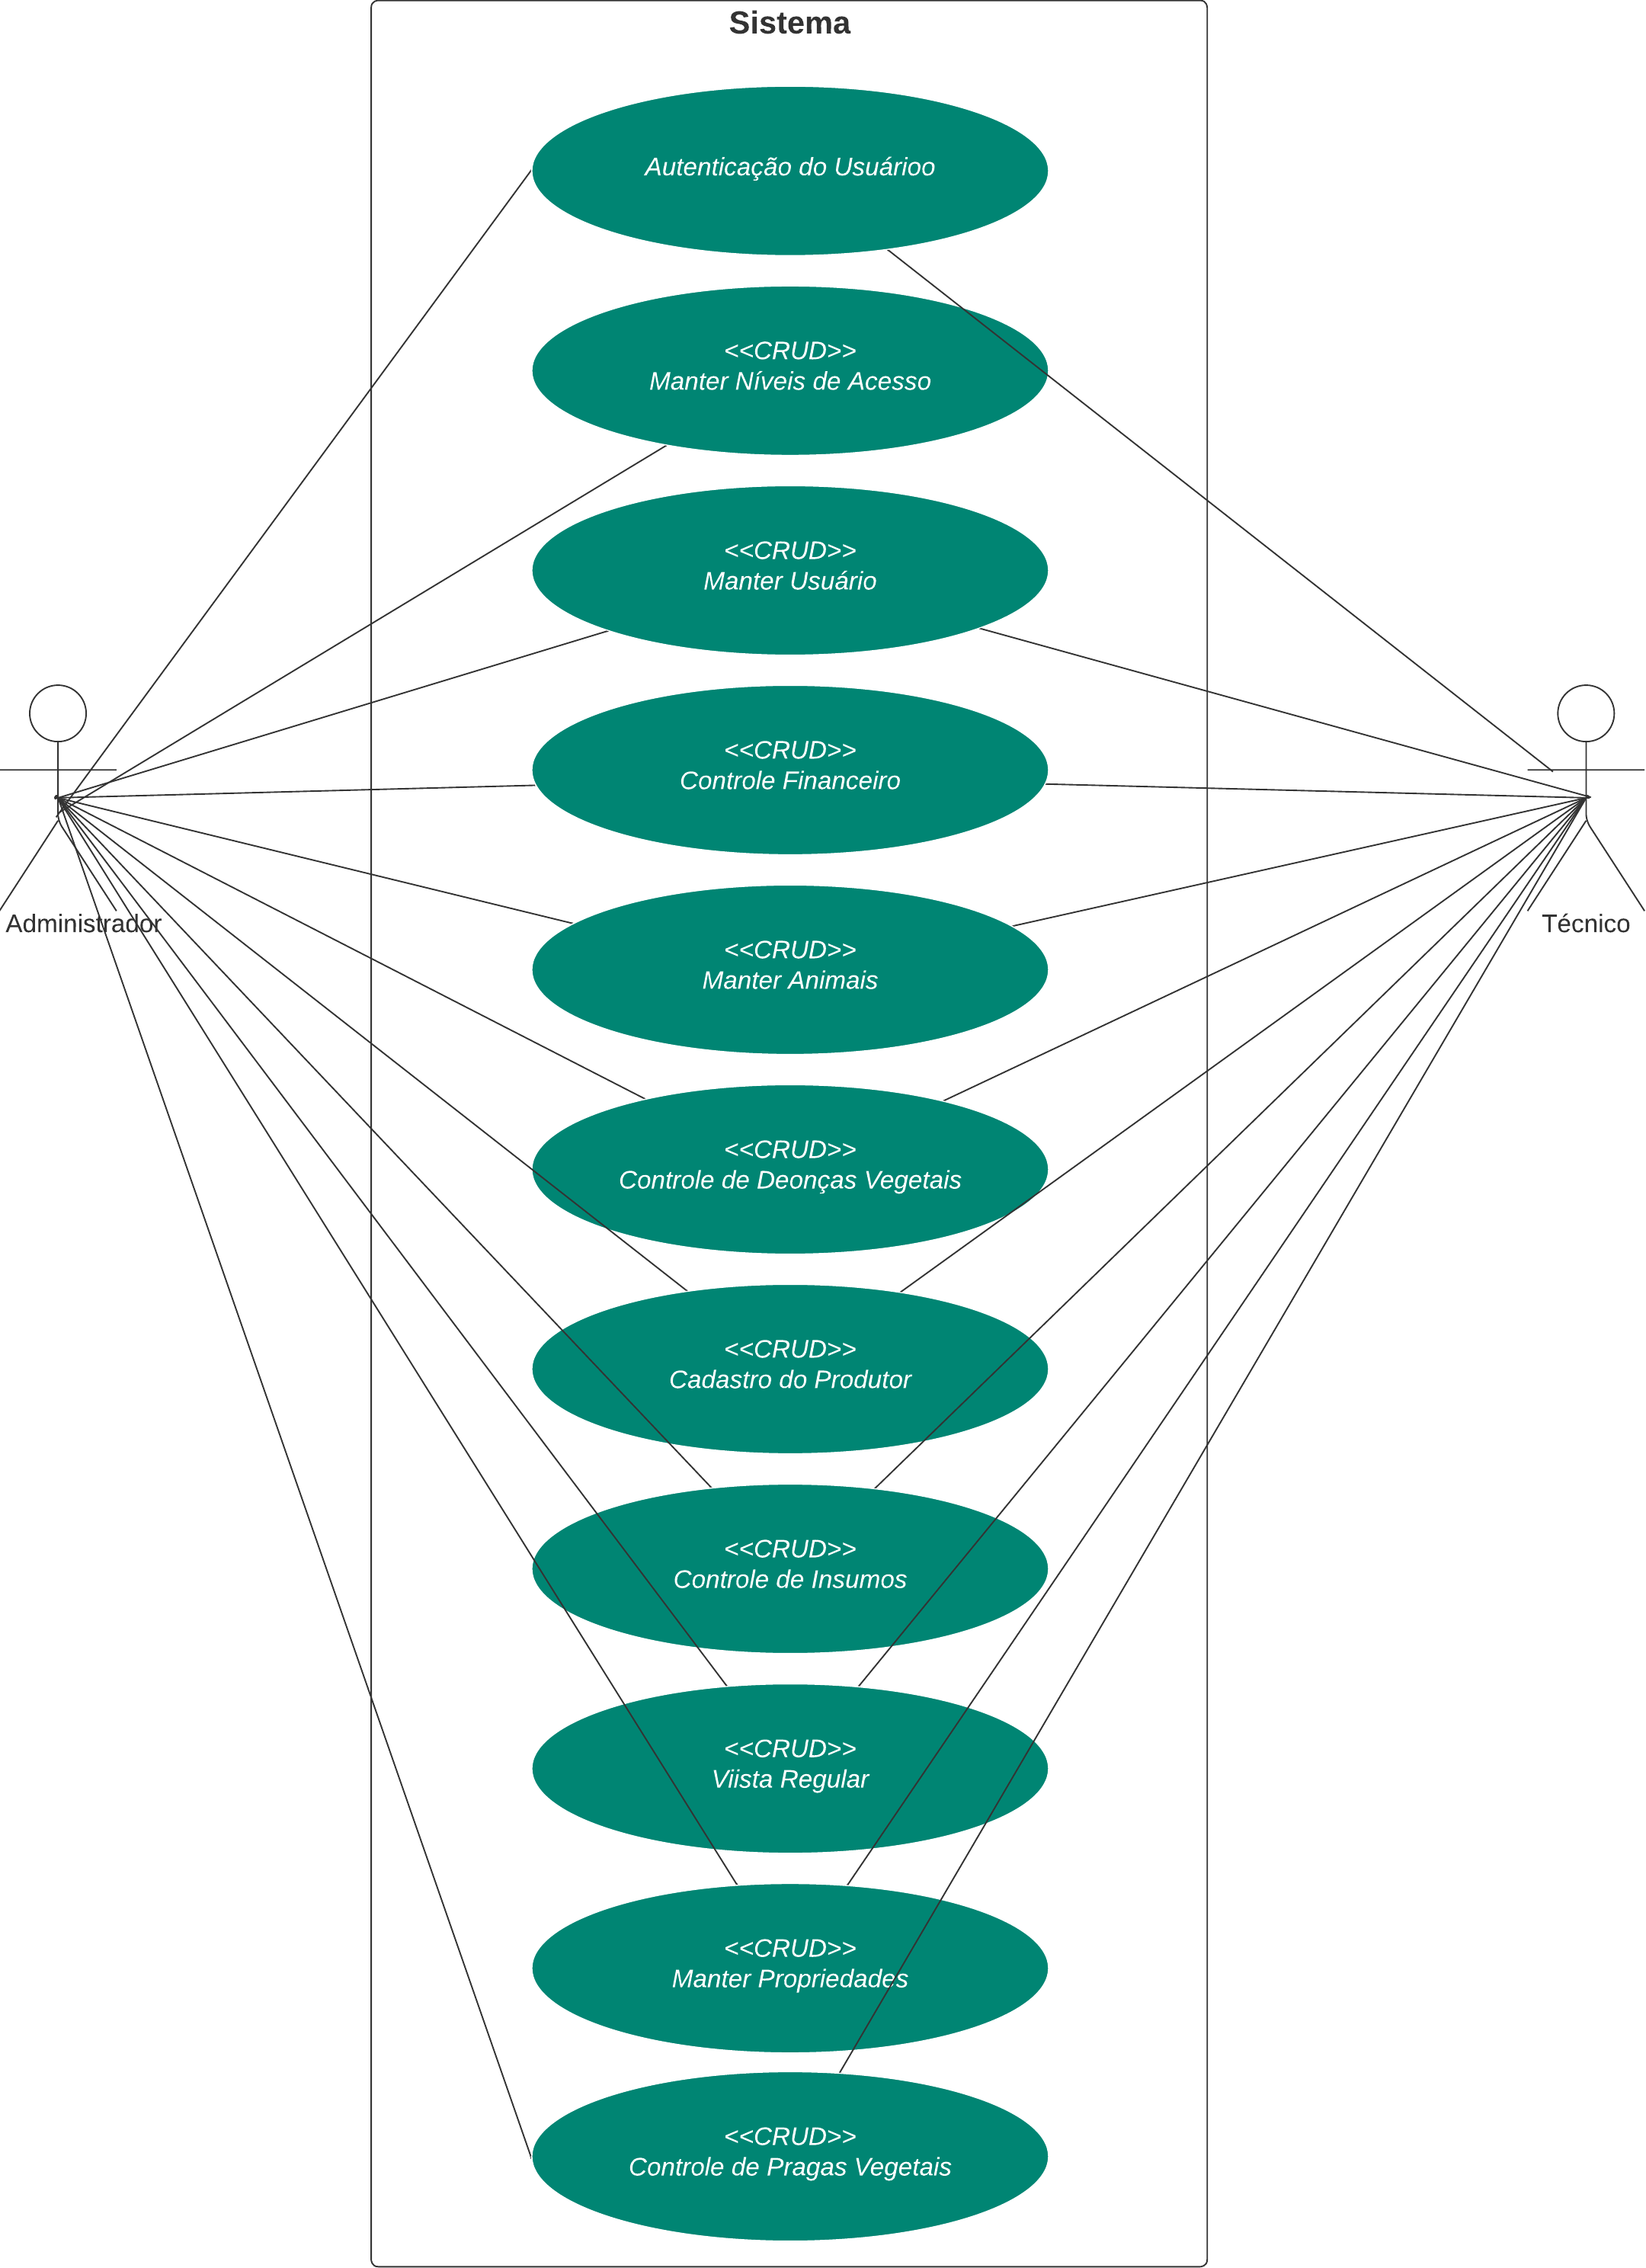
\includegraphics[scale=0.2]{idr-use-case-diagram}
  \fonte{}
\end{figure}

\section{Apresentação do sistema}\label{sec:apresentacaoSistema}

Apresenta as funcionalidades e o uso de recursos tecnológicos do sistema por meio de suas telas, enfatizando a interação com o sistema. A apresentação do sistema é feita sob a forma de texto, com telas e definição de padrões que forem relevantes ao contexto do trabalho. As telas são tratadas como figuras, cópias (print screen) de relatórios ou consultas também são figuras.

A \autoref{fig:cadastroPaciente} exibe a tela de acesso ao Cadastro de Pacientes.

\begin{figure}[htpb]%% Ambiente figure
  \captionsetup{width=0.43\textwidth}
  \caption{Tela de acesso ao Cadastro de Pacientes.}%% Legenda
  \label{fig:cadastroPaciente}%% Rótulo
  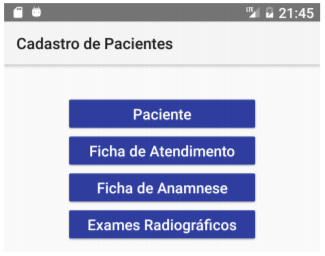
\includegraphics[scale=0.8]{cadastro-paciente}%% Dimensões e localização
  \fonte{}%% Fonte
\end{figure}

\section{Implementação do sistema}\label{sec:implementacaoSistema}

Nesta seção é documentada a implementação do sistema com partes relevantes ou exemplos de código, rotinas, funções. Inclui, ainda, a descrição técnica do uso de recursos (componentes, bibliotecas, etc.) da linguagem. Ressalta-se que cada orientador avaliará juntamente com seu orientado o que poderá ser descrito nesta seção. Isso sem que sejam revelados detalhes do sistema que possam comprometer seu uso comercial ou científico ou que a descrição fique muito sucinta ou superficial.

Em materiais e método estão quais os recursos utilizados, neste capítulo é reportado como esses recursos foram utilizados para resolver o problema.

Sugere-se colocar listagens curtas de código, enfatizando aspectos específicos das tecnologias utilizadas ou da implementação. Sugere-se, ainda, que o código não seja apresentado sob a forma de print screen, e sim copiado e colado no texto, mantendo, se possível, a formatação. Todas as listagens de código devem ser devidamente explicadas. A explicação deve ser técnica, fundamentada em aspectos conceituais e boas práticas de programação.

Enfatizar os diferenciais do sistema: procedimentos armazenados, consultas SQL, uso de componentes, uso de padrões de projeto, a forma de uso dos recursos da linguagem. Esses diferenciais são no sentido de explicitar as vantagens, desvantagens, dificuldades e facilidades que esses recursos impetraram no desenvolvimento do sistema em termos técnicos. Esses diferenciais servirão para avaliar pela utilização ou não desses recursos, pelo menos para sistemas iguais ou semelhantes ao reportado no trabalho.

Reportar a forma como o sistema foi verificado e validado. No sentido de verificar se os requisitos definidos para o mesmo foram atendidos. Os testes podem ser realizados pelo professor orientador, pelos professores que compõem a banca, por pessoas que serviram de base para as informações para o sistema e etc. Os testes podem ser realizados com base em um plano de testes elaborado juntamente com a análise e projeto do sistema. Para validar a implementação podem ser desenvolvidas rotinas de teste unitário.

Se houver implantação do sistema, mesmo que seja para teste, reportar a forma como isso foi feito, a geração de instaladores, os problemas com ambiente e sistema operacional, incluindo banco de dados e outros. Deixar explícito o procedimento para instalar e usar o sistema.

Quando for necessário, citar no texto do trabalho nomes de campos, tabelas ou rotinas específicas utilizadas na implementação de um software, utilizar a fonte courier new para destacar esses nomes.

Um exemplo de listagem de código fonte pode ser observado na \autoref{codigo:classeFoo}, que representa a classe Aluno.

\begin{sourcecode}[htb]
  \caption{\label{codigo:classeFoo}Classe Aluno}
  \begin{lstlisting}[frame=single, language=Java]
@Entity
public class Foo {

    @Id
    @GeneratedValue(strategy = GenerationType.IDENTITY)
    private Long id;

    private String nome;

    private Integer ra;

    // constructor, getters and setters
}
\end{lstlisting}
  \fonte{}
\end{sourcecode}

\section{Discussões (opcional)}\label{sec:discussoes}

O trabalho contém esta seção quando considerado que há resultados (em termos de dados) e discussões relevantes ou suficientes para justificar uma seção. Se existentes e não justificarem uma seção, eles podem estar na seção que relata a implementação do sistema.

Nesta seção estão os resultados obtidos da realização de testes quantitativos e qualitativos, independentemente da quantidade, tipo e volume de testes realizados. Os resultados dos testes são discutidos tendo como base o referencial teórico e os objetivos pretendidos com o trabalho. Esses testes podem resultar de implantação e testes de uso do sistema.
